\section{Results}
\label{sec:results}

We take the regimes in order of how much the model already knows. Each subsection asks one question and ends with what it implies. Table~\ref{tab:main} gives every target-task number for Qwen, and Table~\ref{tab:side} gives every side-effect measure.

\begin{table}[p]
\centering\small
\begin{tabular}{llllr}
\toprule
Method & Programmer & Test acc. [95\% CI] & Test NLL & Dev acc. \\
\midrule
\multicolumn{5}{l}{\textit{SST-5}} \\
Base & -- & 44.9 \tiny[42.8, 46.9] & 3.19 & 42.3 \\
Label prior & -- & 23.1 \tiny[21.4, 24.8] & 1.58 & 25.3 \\
LoRA & -- & 59.0 \tiny[57.0, 61.1] & 0.93 & 57.4 \\
WSP r1 & Fable & 47.3 \tiny[45.2, 49.2] & 1.25 & 47.4 \\
WSP r4 & Fable & 48.0 \tiny[45.9, 50.0] & 1.26 & 46.1 \\
WSP r5 & Fable & 46.7 \tiny[44.5, 48.8] & 1.27 & 46.0 \\
WSP o1 & Opus & \multicolumn{3}{l}{no edit beat base} \\
\multicolumn{5}{l}{\textit{SST-5 inverted}} \\
Base & -- & 4.0 \tiny[3.2, 4.8] & 9.59 & 5.0 \\
Label prior & -- & 23.1 \tiny[21.4, 24.8] & 1.58 & 25.3 \\
LoRA & -- & 49.3 \tiny[47.2, 51.4] & 1.08 & 49.8 \\
WSP r1 & Fable & 46.4 \tiny[44.3, 48.5] & 1.26 & 48.1 \\
WSP r2 & Fable & 46.2 \tiny[44.1, 48.3] & 1.26 & 44.2 \\
WSP r3 & Fable & 48.1 \tiny[46.0, 50.1] & 1.23 & 48.4 \\
WSP o1 & Opus & 45.7 \tiny[43.7, 47.7] & 1.24 & 44.8 \\
\multicolumn{5}{l}{\textit{Twin-2K}} \\
Base & -- & 30.9 \tiny[29.4, 32.4] & 2.60 & 29.4 \\
Label prior & -- & 47.1 \tiny[45.4, 48.6] & 1.29 & 47.8 \\
LoRA & -- & 42.8 \tiny[41.2, 44.4] & 1.36 & 40.6 \\
WSP r1 & Fable* & 32.8 \tiny[31.3, 34.2] & 1.51 & 33.2 \\
WSP r2 & Fable & 45.0 \tiny[43.4, 46.6] & 1.38 & 45.8 \\
WSP o1 & Opus & 31.9 \tiny[30.4, 33.3] & 1.52 & 31.7 \\
WSP p1 & Fable, preserve & 35.2 \tiny[33.7, 36.8] & 2.90 & 35.0 \\
\multicolumn{5}{l}{\textit{Fictional facts}} \\
Base & -- & 21.1 \tiny[18.4, 23.7] & 3.46 & 19.4 \\
Label prior & -- & 27.4 \tiny[24.6, 30.4] & 1.59 & 24.1 \\
LoRA & -- & 98.8 \tiny[98.0, 99.4] & 0.10 & 99.2 \\
WSP r1 & Fable & 100.0 \tiny[100.0, 100.0] & 0.00 & 100.0 \\
WSP r2 & Fable & 100.0 \tiny[100.0, 100.0] & 0.01 & 100.0 \\
WSP r4 & Fable & 100.0 \tiny[100.0, 100.0] & 0.00 & 100.0 \\
WSP o1 & Opus & 76.9 \tiny[74.0, 79.4] & 1.03 & 73.0 \\
WSP p1 & Fable, preserve & 25.0 \tiny[22.2, 27.7] & 2.81 & 25.2 \\
\bottomrule
\end{tabular}

\caption{Accuracy (\%) and NLL on Qwen2.5-1.5B. Test accuracy carries a bootstrap 95\% interval. WSP runs \texttt{r}$n$ were programmed by Fable and \texttt{o1} by Opus. \texttt{p1} used the preserve brief. *Twin-2K \texttt{r1} used Fable 5.1 and an earlier brief that discouraged item-level tables; its dev figure is the programmer's own. For runs scored only on test by us, dev is the programmer's full-dev measurement, recomputed by the auditor. LoRA is seed 0; Table~\ref{tab:reliability} gives the other seeds. For facts, LoRA is the fifteen-epoch configuration (Section~\ref{sec:compile}).}
\label{tab:main}
\end{table}

\subsection{Redirect: can programming fix a model that knows but misreads?}
\label{sec:redirect}
SST-5 inverted is built to answer this. The base model scores 4.0\%, far below the 20\% chance level. It is not confused: it confidently picks the true sentiment, which is now always wrong. The probe reads the correct mirrored answer 40.8\% of the time from the same activations, so the knowledge is intact.

\paragraph{Every programmer found the same fix.}
\begin{itemize}
  \item \textbf{Who tried.} Four programmers attempted this task on Qwen (three Fable, one Opus), and one on SmolLM2.
  \item \textbf{What they all did.} Each option line reads ``very negative'', ``negative'', ``neutral'', ``positive'' or ``very positive''. Mirroring the labels is therefore the same as exchanging the words ``negative'' and ``positive''. Each is a single token, so swapping their two rows in the embedding matrix makes every option \emph{read} as its mirror image. The model then does exactly what it did before, matching the review's sentiment to the option text, and lands on the mirrored answer.
  \item \textbf{How much the swap alone does.} It moves dev accuracy from 5.0\% to 44.2--44.3\% in the runs that measured it separately.
  \item \textbf{The finishing touches.} Small additions brought the final Qwen edits to 45.7--48.1\% on test: a temperature rescale against overconfidence, a nudge that lets ``neutral'' be chosen again, and in one run a rank-one intensity correction.
\end{itemize}

\paragraph{The effect is the swap, and it is specific.} Two controls settle this.
\begin{itemize}
  \item Swapping `` negative'' and `` positive'' with no other change scores 46.2\% on test. That is essentially the full Fable \texttt{r1} edit (46.4\%).
  \item Swapping two sentiment-unrelated words (`` table'', `` river'') leaves the model at 4.0\%, exactly where it started.
  \item The same pattern holds on SmolLM2: the swap alone takes it from 11.4\% to 38.6\%, the final edit reaches 45.4\%, and the unrelated swap does nothing (Table~\ref{tab:smollm}).
\end{itemize}

\paragraph{The swap is as good as LoRA and more reliable than its default configuration.}
\begin{itemize}
  \item \textbf{Seed 0: a statistical tie.} LoRA reached 49.3\% with seed 0. The best programmed edit (48.1\%) is not significantly different from it (paired bootstrap, $p=0.37$). The other three are 2.9--3.6 points lower ($p\le0.023$).
  \item \textbf{Other seeds: LoRA mostly fails.} Seeds 1 and 2 never learned the task: 23.9\% and 27.7\% (Table~\ref{tab:reliability}). Training starts confidently wrong (loss 3.9), falls to the uniform-guess plateau ($\ln 5\approx1.61$), and stays there.
  \item \textbf{Seed 0 barely escaped.} It sat on the same plateau for about 200 of its 500 batches. Rerunning it with the same settings as seeds 1--2 reproduced 49.5\%, so the failures are not an artefact of a configuration change.
  \item \textbf{The same failure on SmolLM2.} Its LoRA runs stuck on the same plateau on all three seeds (21.5--22.7\%).
  \item \textbf{More steps get LoRA out; a larger step size does not.} On Qwen, with three times the data (12,000 examples, so three times the steps), all three seeds escaped the plateau between batches 250 and 750 of 1,500 and reached 58.1--61.2\%. With a three times larger learning rate, all three stayed on it (19.4--20.0\%; Table~\ref{tab:plateau}). We tried neither change on SmolLM2.
\end{itemize}
Programming found the fix in every one of its five attempts.

\paragraph{With few labels, programming wins.} With only 256 distinct training examples, LoRA reaches 29.1\% (Table~\ref{tab:reliability}). It needs about 1,024 to pass the programmed edits.

\paragraph{The one weakness.} The redirection edits leave the model's position habits alone. Only 11--20\% of test questions get the same answer in every option rotation, against 66\% after LoRA. The swap changes what the model reads, not how it weighs positions.

\paragraph{Takeaway.} When a model has the knowledge and only its readout is wrong, programming finds a fix that is tiny (as few as 4,608 changed weights out of 1.5 billion), readable in one sentence, reproducible across independent attempts and across model families, and more reliable than default fine-tuning.

\begin{table}[t]
\centering\small
\begin{tabular}{lccccc}
\toprule
Task & LoRA seeds 0 / 1 / 2 & $n=256$ & $n=1{,}024$ & full pool & WSP (all runs) \\
\midrule
SST-5 & 59.0 / 56.6 / 58.1 & 54.2 & 57.8 & 59.0 & 46.7--48.0 \\
SST-5 inverted & 49.3 / 23.9 / 27.7 & 29.1 & 53.1 & 49.3 & 45.7--48.1 \\
\bottomrule
\end{tabular}

\caption{How reliable LoRA is, and how much data it needs (Qwen, test accuracy, \%). Seeds use the default configuration (4,000 examples, 250 optimizer steps). The learning curve keeps 250 optimizer steps but draws them from only $n$ distinct training examples (seed 0). The last column is the range over all programmed edits for the task.}
\label{tab:reliability}
\end{table}

\subsection{Compile: can programming add knowledge the model lacks?}
\label{sec:compile}
The fictional facts task answers this. Neither the base model (21.1\%) nor the probe (21.0\%) knows anything about the 300 invented people. We expected programming to fail here and fine-tuning to succeed. At first the opposite happened.

\paragraph{Fine-tuning needed far more training than expected.}
\begin{itemize}
  \item \textbf{The default failed.} With 4,000 examples (about 1.5 epochs), LoRA did not learn at all: its loss stayed at $\ln 5$ and test accuracy was 22.2\%. Higher learning rates also failed.
  \item \textbf{A smaller version showed LoRA can do it.} On a 60-person version, about fifteen epochs at learning rate $10^{-4}$ reached 96.7\% under an unseen wording.
  \item \textbf{Fifteen epochs on the full task worked.} LoRA reached 98.8\% after 40,500 examples and 3.6 T4-hours.
\end{itemize}
This matches earlier evidence that fine-tuned models need many exposures before a new fact can be retrieved under new phrasing~\citep{allenzhu2023physics}. Every configuration is in Appendix~\ref{app:facts-lora}.

\paragraph{Fable built a lookup machine, three times.} All three standard Fable runs looked for something in the model to amplify, found nothing, and changed strategy. Each built an explicit lookup circuit from the training labels in the first two layers:
\begin{itemize}
  \item name tokens receive codes in directions no prompt token uses;
  \item layer-0 attention heads pool those codes into a ``bag'' that identifies the person;
  \item one layer-0 MLP neuron per fact fires on that bag and writes the true value;
  \item a layer-1 head copies the matching option's letter to the answer position.
\end{itemize}
Each scored 100\% on test, under a question wording none of them had designed against, using 6, 10 and 17 forward passes. The fact table driving each circuit comes from the training labels, which every programmer disclosed as the brief requires. On SmolLM2 the Fable programmer built the same kind of circuit, with the same result: 100\% on test in four passes.

\paragraph{Opus wrote into the model's own memory.} The Opus run took a route close to ROME~\citep{meng2022rome}, which treats mid-layer MLPs as key--value memories.
\begin{itemize}
  \item \textbf{Keys.} Each person's layer-8 MLP input at their name tokens.
  \item \textbf{Values.} Each answer's typical activation at its option token.
  \item \textbf{The edit.} It repurposed 900 layer-8 neurons to map one to the other.
\end{itemize}
Writing all three facts at one position overloaded it, so the final edit spreads them over the last three name tokens. It reached 76.9\% on test.

\paragraph{The same pattern on real data.} On Twin-2K, the base model scores 30.9\%. Simply predicting each question's most common training answer, ignoring the person entirely, scores 47.1\%, and LoRA gains twelve points (42.8\%).
\begin{itemize}
  \item \textbf{Fable compiled the prior into a circuit.} The circuit spans the first three layers and reached 45.0\%, 2.3 points above LoRA (paired bootstrap, $p=0.008$) and close to the prior itself. It uses no information about the person.
  \item \textbf{Opus had the same idea, at small scale.} It put per-option offsets from training counts into a single repurposed neuron and gained one point (31.9\%).
\end{itemize}
A second standard-brief Fable run (\texttt{r4}) re-weighted the option-reading attention heads instead, reaching 37.0\% with the model intact. We exclude it from the main comparison because its read-out is mathematically a regression fitted to the training labels, which the brief forbids. It is reported in full in Appendix~\ref{app:deviations}, and including it would not change any conclusion.

\paragraph{Takeaway.} Programming \emph{can} add knowledge the model does not have, but not by learning. It compiles: the programmer turns the training labels into a table and builds machinery to look it up. On facts this was faster and more accurate than fine-tuning.

\subsection{The catch: what does a compiled circuit cost the rest of the model?}
\label{sec:catch}
A model that recalls 900 invented facts perfectly sounds like a clear win. Figure~\ref{fig:tradeoff} and Table~\ref{tab:side} show what it costs.

\begin{table}[p]
\centering\scriptsize
\resizebox{\linewidth}{!}{\begin{tabular}{llllrrrr}
\toprule
Task & Method & Edit type & Consistent & Other task & MMLU & Top-1 & Rescaled NLL \\
\midrule
SST-5 & Base & -- & 14.0 & 29.4 & 59.6 & 45.9 & 2.77 \\
 & LoRA & -- & 72.3 & 32.3 & 60.4 & 45.8 & 2.76 \\
 & WSP r1 (Fable) & through & 18.0 & 30.5 & 52.4 & 45.8 & 2.78 \\
 & WSP r4 (Fable) & through & 6.7 & 31.2 & 60.0 & 45.8 & 2.79 \\
 & WSP r5 (Fable) & through & 14.0 & 30.2 & 58.6 & 45.2 & 2.84 \\
SST-5 inverted & Base & -- & 15.3 & -- & 59.6 & 45.9 & 2.77 \\
 & LoRA & -- & 65.7 & -- & 55.6 & 45.9 & 2.76 \\
 & WSP r1 (Fable) & through & 20.0 & -- & 57.8 & 45.8 & 2.79 \\
 & WSP r2 (Fable) & through & 15.0 & -- & 59.4 & 45.8 & 2.78 \\
 & WSP r3 (Fable) & through & 17.0 & -- & 54.8 & 45.5 & 2.83 \\
 & WSP o1 (Opus) & through & 11.0 & -- & 59.4 & 45.8 & 2.78 \\
Twin-2K & Base & -- & 23.0 & 42.3 & 59.6 & 45.9 & 2.77 \\
 & LoRA & -- & 41.0 & 43.3 & 60.0 & 45.7 & 2.77 \\
 & WSP r1 (Fable*) & through & 24.0 & -- & 59.6 & 45.7 & 2.79 \\
 & WSP r2 (Fable) & bypass & 89.3 & 19.9 & 23.4 & 0.1 & 11.86 \\
 & WSP o1 (Opus) & through & 20.7 & 43.6 & 58.0 & 45.8 & 2.78 \\
 & WSP p1 (Fable, preserve) & through & 40.0 & 42.2 & 57.6 & 45.8 & 2.77 \\
Fictional facts & Base & -- & 12.0 & 42.3 & 59.6 & 45.9 & 2.77 \\
 & LoRA & -- & 97.0 & 45.9 & 62.0 & 45.6 & 2.78 \\
 & WSP r1 (Fable) & bypass & 100.0 & 18.7 & 22.2 & 0.0 & -- \\
 & WSP r2 (Fable) & bypass & 100.0 & 19.2 & 25.2 & 0.0 & 11.97 \\
 & WSP r4 (Fable) & bypass & 100.0 & 20.0 & 25.8 & 0.0 & -- \\
 & WSP o1 (Opus) & through & 65.7 & 42.2 & 59.6 & 45.6 & 2.78 \\
 & WSP p1 (Fable, preserve) & through & 1.7 & 38.1 & 55.6 & 39.6 & 3.41 \\
\bottomrule
\end{tabular}
}
\caption{What each change costs (Qwen). \emph{Edit type}: \emph{bypass} edits overwrite early-layer computation with a hand-built circuit; \emph{through} edits act through the model's existing pathways. \emph{Consistent}: share of 300 test questions answered with the same option text in all five option rotations (\%). \emph{Other task}: dev accuracy on SST-5 for Twin-2K and facts edits (unedited 42.3), and on Twin-2K for SST-5 edits (unedited 29.4); for preserve runs this is the full preserve set. \emph{MMLU}: 500 zero-shot questions (unedited 59.6, chance 25). \emph{Top-1}: next-token accuracy on WikiText-2 (unedited 45.9). \emph{Rescaled NLL}: WikiText-2 NLL after the best single logit rescale (unedited 2.77; ``--'' means it overflows).}
\label{tab:side}
\end{table}

\paragraph{Bypass circuits destroy the model.} After any of the three Fable facts circuits, or the Twin-2K circuit:
\begin{itemize}
  \item MMLU falls from 59.6\% to 22.2--25.8\%, chance level for four options.
  \item Next-token top-1 accuracy on ordinary text falls from 45.9\% to 0.0--0.1\%.
  \item No temperature rescale recovers the language-modelling loss, and in two cases the loss overflows.
  \item On SST-5, one facts circuit sends 94\% of answers to the same letter.
\end{itemize}
The SmolLM2 facts circuit does the same: MMLU 22.6\% (unedited 48.8\%) and top-1 0.0\%.

\paragraph{Through edits mostly keep the model intact.} The Opus facts memory leaves MMLU at 59.6\% and top-1 at 45.6\%; LoRA leaves them at 62.0\% and 45.6\%. Every SST-5, SST-5-inverted and Twin-2K through edit keeps top-1 within 0.7 points of the unedited model. The one exception is the facts preserve run (Section~\ref{sec:preserve}).

\paragraph{Why bypass circuits do this.} To build a reliable lookup, the programmer rewired layer-0 attention heads that every token passes through. Its final write into the residual stream is large (a norm of 16,000 to 40,000 in different runs) and drowns out whatever the rest of the network computes. The circuit does not sit alongside the model's normal behaviour; it replaces it. The Opus edit instead reuses an existing pathway, and LoRA's low-rank updates are spread across layers. Both add to the model's computation rather than override it.

\paragraph{A trap in the other direction.} Measured by raw perplexity, nearly every through edit looks badly damaged too: WikiText perplexity rises from 15.9 to between 1,800 and 6,300. That rise is the temperature most of these edits include, which multiplies every logit by a constant. Top-1 accuracy is unchanged, and one rescale brings the loss back to the unedited level (2.78--2.84, against 2.77). Raw perplexity would have condemned harmless edits.

\paragraph{Takeaway.} Judged by task accuracy alone, the best programming results are also the most destructive. Judged by raw perplexity, harmless edits look destructive. Evaluating an edit needs a measure of general ability that a temperature change cannot fake.

\subsection{Can a programmer compile without breaking the model?}
\label{sec:preserve}
The standard brief never asked the programmer to protect anything, and in every compliant compile-task run on Qwen, the strongest programmer took the destructive route. Is that a limit of the method, or of the instruction? We ran the preserve brief on the two compile tasks.

\paragraph{Twin-2K: yes, at a price.}
\begin{itemize}
  \item \textbf{A different kind of edit.} Under the preserve brief, Fable built no circuit. It found that a few layer-21 attention heads choose the answer by reading the option text. To each of them it added a gated, rank-3 change: at the answer position of an agree-scale, support-scale or money-split question, attention shifts toward the kind of option people usually choose. Elsewhere the gate is closed.
  \item \textbf{Accuracy.} The edit reached 35.2\% on test, 4.3 points above the unedited model.
  \item \textbf{What it costs.} SST-5 accuracy is 42.2\% (unedited 42.3\%), and 41.4\% on the preserve examples the programmer never used. WikiText top-1 and loss are unchanged, and MMLU is 2 points lower (57.6\%).
  \item \textbf{Consistency.} It also answered consistently under option rotation more often than any other Twin-2K edit except the bypass circuit (40\%, against 21\% for the Opus edit).
\end{itemize}
Compared with the bypass circuit, it keeps about a third of the gain and almost all of the model.

\paragraph{Facts: no.} The preserve run spent 49 of its 50 passes building a gated person memory that stays silent on other text.
\begin{itemize}
  \item \textbf{Accuracy.} Its best edit raised test accuracy only from 21.1\% to 25.0\%. On the dev questions it had not used for selection, the gain was about 4 points.
  \item \textbf{The preserve check.} The edit failed the bar (38.1\% against 40\%).
  \item \textbf{General ability.} It did real but partial damage: MMLU 55.6\%, top-1 39.6\%, and a loss no rescale recovers.
  \item \textbf{Where the damage comes from.} The programmer traced it to the constant signal its gates needed. Signals that later layers damp unpredictably are hard to cancel exactly.
\end{itemize}

\paragraph{Takeaway.} The brief, not the method, decides whether an edit goes around the network or through it. Preserving the model costs most of the compiled gain, and on a task with nothing to build on, the programmer could not find an edit that both added knowledge and preserved the model. Any brief should state what must be preserved, and any evaluation should check it.

\subsection{Learn: where does programming fall short?}
\label{sec:learn}
On standard SST-5 the model already does reasonably well (44.9\%), and the probe finds only a little unused information (+5.6 points). There is nothing to redirect and no table to write down. Improving requires a better mapping from review to sentiment level.

\paragraph{Three programmers, three mechanisms, one ceiling.} Three independent Fable runs found three different mechanisms:
\begin{itemize}
  \item a hand-built circuit (47.3\%);
  \item one repurposed MLP neuron that shifts the class prior (48.0\%);
  \item constant steering through attention value biases (46.7\%).
\end{itemize}
All three fix the same defect. The model almost never answers ``neutral'' (1.5\% of its predictions, against 18\% of labels) and over-uses ``very''. An offline estimate by one programmer puts the ceiling for any such prior shift near 50\%. The Opus run found no edit that beat the base model.

\paragraph{LoRA does far better, with any amount of data.} LoRA reached 59.0\% (56.6--59.0\% over three seeds). Its advantage is not more data. With only 256 distinct training examples, a tenth of what a programmer reads, LoRA still reached 54.2\% (Table~\ref{tab:reliability}). The bottleneck is the mapping itself. The conversion from the model's sentiment representation to the right letter is spread across attention heads in layers 21--26, and no small, readable change moves it far.

\paragraph{Takeaway.} When the improvement has to be learned from examples rather than written down, fine-tuning wins clearly, and the reason is not data.

\subsection{Does it hold on another model?}
\label{sec:smollm}
Table~\ref{tab:smollm} repeats the central experiments on SmolLM2-1.7B-Instruct.
\begin{itemize}
  \item \textbf{The knowledge map is the same.} The probe finds large headroom on SST-5 inverted (+25 points) and almost none on SST-5 or facts.
  \item \textbf{The redirect regime replicates.} The programmer independently found the same embedding swap. The final edit reached 45.4\% from 11.4\%, with MMLU and top-1 unchanged. Default LoRA stuck on the plateau on all three seeds (21.5--22.7\%).
  \item \textbf{The compile regime replicates, damage included.} The programmer built a layer-0/1 lookup circuit that scored 100\% on test and reduced the model to chance on MMLU, with 0\% top-1.
  \item \textbf{The combination replicates.} LoRA trained on top of the final SST-5-inverted edit reached 55.9--56.6\% on every seed (Section~\ref{sec:combine}).
\end{itemize}

\begin{table}[t]
\centering\small
\begin{tabular}{llccc}
\toprule
Method & Edit type & Test acc. & MMLU & Top-1 \\
\midrule
Base model & -- & -- & 48.8 & 46.0 \\
\multicolumn{5}{l}{\textit{SST-5 inverted}: base 11.4, probe headroom +25.0} \\
\quad LoRA (seed 0) & -- & 22.7 & -- & -- \\
\quad Control: swap two unrelated words & -- & 11.4 & -- & -- \\
\quad WSP f1, embedding swap alone & through & 38.6 & -- & -- \\
\quad WSP f1, final edit & through & 45.4 & 48.8 & 46.0 \\
\multicolumn{5}{l}{\textit{Fictional facts}: base 21.8, probe headroom +1.7} \\
\quad WSP f1, final edit & bypass & 100.0 & 22.6 & 0.0 \\
\multicolumn{5}{l}{\textit{SST-5}: base 36.9, probe headroom +1.9} \\
\bottomrule
\end{tabular}

\caption{The second model family: SmolLM2-1.7B-Instruct (test accuracy, \%). MMLU and top-1 are general-ability measures as in Table~\ref{tab:side} (unedited: 48.8 and 46.0). The final SST-5-inverted edit adds a label-free letter-bias correction and a temperature to the embedding swap. For LoRA on top of it, MMLU and top-1 are ranges over the three seeds.}
\label{tab:smollm}
\end{table}

\subsection{Programming, then fine-tuning}
\label{sec:combine}
The regimes suggest the two methods fail in different places. Can they cover for each other? We trained LoRA, with the default configuration and 4,000 examples, on top of two programmed edits, over three seeds (Table~\ref{tab:combine}, Figure~\ref{fig:combination}). On SST-5 inverted we also checked what the edit does that tuning LoRA cannot (Table~\ref{tab:plateau}).

\paragraph{Facts.} Starting from the Opus memory edit (76.9\% alone), LoRA reached 99.0--99.7\% on test.
\begin{itemize}
  \item \textbf{Against LoRA alone, same budget.} From the base model, the same budget gave 22.2\%.
  \item \textbf{Against LoRA alone, any budget.} LoRA reached 98.8\% with about ten times the training presentations and 3.6 GPU-hours. At the default learning rate we tried no budget in between, so the saving may be smaller.
  \item \textbf{How fast it learned.} Training loss fell to 0.07 within 100 steps. The edit gives LoRA a working person-to-fact memory to refine, instead of one to discover.
\end{itemize}

\paragraph{SST-5 inverted.} Starting from the Fable swap edit (46.4\% alone), LoRA reached 57.3--58.5\% on every seed.
\begin{itemize}
  \item \textbf{Against LoRA alone, same budget.} 23.9--49.3\%, learning on one seed of three.
  \item \textbf{Against LoRA alone, more data.} With three times the data (Qwen only), LoRA alone learned on every seed and reached 58.1--61.2\% (mean 60.0\%, against 58.0\% for the combination). The edit saves data; it does not raise the ceiling. We did not train the combination on the larger budget.
  \item \textbf{The swap is what matters.} LoRA on a hand-written swap of the two label words (46.2\% alone) reached 57.6--58.5\%, the same as on the programmer's full edit. Once LoRA trains, the programmer's further changes add nothing; its contribution was finding the swap.
  \item \textbf{It replicates on SmolLM2.} LoRA alone stuck on all three seeds (21.5--22.7\%). On top of the Fable edit (45.4\% alone) it reached 55.9--56.6\% on every seed.
  \item \textbf{Why it helps.} The edit removes the confidently-wrong start, so LoRA does not spend its steps escaping the plateau. LoRA then improves the sentiment mapping well beyond what the edit can.
\end{itemize}

\begin{table}[t]
\centering\small
\resizebox{\linewidth}{!}{\begin{tabular}{llccccc}
\toprule
Task & Starting edit & Edit alone & LoRA alone & Edit, then LoRA & MMLU, edit then LoRA & LoRA, 10$\times$ data \\
\midrule
Fictional facts & Opus memory edit (o1) & 76.9 & 22.2 & 99.3 / 99.7 / 99.0 & 58.2 / 58.0 / 59.6 & 98.8$^\ddagger$ \\
SST-5 inverted & Fable swap edit (r1) & 46.4 & 49.3 / 23.9 / 27.7 & 58.2 / 57.3 / 58.5 & 58.6 / 58.0 / 58.2 & -- \\
\bottomrule
\end{tabular}
}
\caption{Programming, then fine-tuning (Qwen, test accuracy, \%). LoRA uses the default configuration (4,000 examples, 250 optimizer steps); values separated by ``/'' are seeds 0, 1 and 2. The MMLU column is for the edit-then-LoRA models (base model 59.6). $^\ddagger$Fifteen epochs (40,500 examples, 3.6 T4-hours). $^\S$12,000 examples, three times the default.}
\label{tab:combine}
\end{table}

\begin{table}[t]
\centering\small
\resizebox{\linewidth}{!}{\begin{tabular}{lclcc}
\toprule
LoRA starts from & Start & LoRA training & Seeds 0 / 1 / 2 & Mean \\
\midrule
\multicolumn{5}{l}{\textit{Qwen2.5-1.5B}} \\
\quad Base model & 4.0 & 4,000 examples & 49.3 / 23.9 / 27.7 & 33.6 \\
\quad Base model & 4.0 & 4,000 examples, learning rate $3\times10^{-4}$ & 19.4 / 19.5 / 20.0 & 19.6 \\
\quad Base model & 4.0 & 12,000 examples & 60.5 / 61.2 / 58.1 & 60.0 \\
\quad Fable swap edit (r1) & 46.4 & 4,000 examples & 58.2 / 57.3 / 58.5 & 58.0 \\
\quad Hand-written label swap & 46.2 & 4,000 examples & 58.5 / 57.6 / 58.0 & 58.0 \\
\multicolumn{5}{l}{\textit{SmolLM2-1.7B}} \\
\quad Base model & 11.4 & 4,000 examples & 22.7 / 21.5 / 22.3 & 22.2 \\
\quad Fable edit (f1) & 45.4 & 4,000 examples & 55.9 / 56.6 / 56.1 & 56.2 \\
\bottomrule
\end{tabular}
}
\caption{Getting LoRA past the SST-5-inverted plateau (Qwen, test accuracy, \%). \emph{Start}: accuracy before LoRA. LoRA uses the default configuration unless stated; 12,000 examples means three times the optimizer steps. The hand-written swap exchanges the embedding rows of `` negative'' and `` positive'' and changes nothing else.}
\label{tab:plateau}
\end{table}

\begin{figure}[t]
\centering
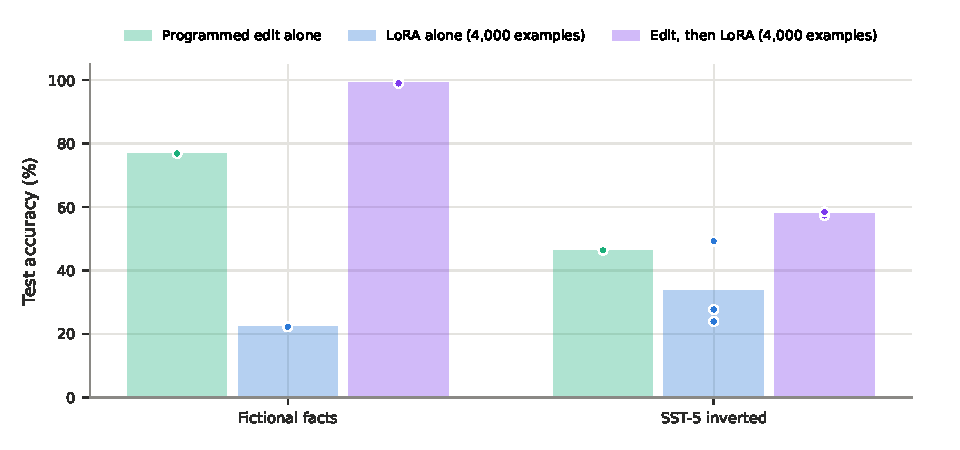
\includegraphics[width=0.8\linewidth]{figures/combination.pdf}
\caption{A programmed edit saves fine-tuning data (Qwen, test accuracy). With 4,000 examples, LoRA from the edit reaches about what LoRA alone reaches with ten times (facts) or three times (SST-5 inverted) the data. Bars are means; dots are individual seeds.}
\label{fig:combination}
\end{figure}

\paragraph{Side effects.} The combined models kept general ability (Table~\ref{tab:combine}).
\begin{itemize}
  \item \textbf{Facts.} MMLU was 58.0--59.6\% over the three seeds (base and edit alone 59.6\%), next-token top-1 45.5\% (base 45.9\%), and accuracy on SST-5 dev 42.6--43.6\% (base 42.3\%).
  \item \textbf{SST-5 inverted.} MMLU was 58.0--58.6\% (edit alone 57.8\%, LoRA alone 55.6\%) and top-1 45.7--45.8\%. Raw perplexity stays high only because of the swap edit's temperature change; one logit rescaling removes it (rescaled NLL 2.79, base 2.77). On SmolLM2, MMLU was 46.6--48.0\% (base 48.8\%) and top-1 46.0\% (base 46.0\%).
\end{itemize}
Every MMLU difference is within its 95\% interval of about $\pm4$ points. \citet{yang2026writing} saw the opposite when they trained LoRA on top of a written patch: the adapter broke neighbouring tasks, as it did when trained from the base model.

\paragraph{Takeaway.} The methods are complements. A programmed edit is cheap and readable but limited. Fine-tuning is general but slow to store new facts and can stall on a confidently wrong start. A programmed edit worked around both of fine-tuning's failure modes we saw, and fine-tuning took both edits well past what programming alone reached. More data fixes both failures too, so what the edit buys is training data: about ten times less on facts and three times less on SST-5 inverted, for about the same final accuracy.

\subsection{Does the programmer matter, and what does programming cost?}
\label{sec:programmer}
\paragraph{The programmer matters when there is something to build.} With the same brief, Fable and Opus did equally well where the fix was a small redirection: 46.2--48.1\% against 45.7\% on SST-5 inverted. Where an edit had to be built, they diverged:
\begin{itemize}
  \item \textbf{Facts.} Fable reached 100\% with bypass circuits; Opus reached 76.9\% through the model's memory.
  \item \textbf{Twin-2K.} Fable reached 45.0\%; Opus reached 31.9\%.
  \item \textbf{SST-5.} Opus found no improving edit at all.
\end{itemize}
Part of the gap is infrastructure: two Opus runs ended early while waiting hours for a GPU. But the direction is what one would expect. Redirection is a small search; building a working circuit is a demanding engineering job.

\paragraph{Cost.} The two methods spend different resources (Appendix Table~\ref{tab:cost}).
\begin{itemize}
  \item \textbf{GPU time.} A programming run scores at most 25,600 examples: minutes of GPU time for short prompts, and about 1.5 T4-hours at most for Twin-2K. LoRA took 29 minutes of T4 time per SST-5 task, 3.6 hours for facts and 5.7 hours for Twin-2K.
  \item \textbf{Programmer API time.} At list prices, a completed programming run cost \$16--\$86, with the two preserve runs higher (\$103 and \$364). An audit cost \$1--\$14.
\end{itemize}
Programming trades GPU hours for frontier-model time. Which is cheaper depends on what each costs you. Combined with fine-tuning, however, a programmed edit cut the GPU time needed on facts by up to tenfold.
